\documentclass[aspectratio=169]{beamer}

\mode<presentation>
\usetheme{Boadilla}
\definecolor{Khaki}{RGB}{144,110,62}
\definecolor{blue}{RGB}{30,90,205}
\definecolor{red}{RGB}{213,94,0}
\definecolor{green}{RGB}{0,128,0}
\setbeamercolor{title}{fg=Khaki}
\setbeamercolor{frametitle}{fg=Khaki}
\setbeamercolor{block title}{bg=Khaki, fg=white}
\setbeamercolor{block body}{bg=white}
\setbeamercolor{structure}{fg=Khaki}
\setbeamercolor{item projected}{fg=white}
\setbeamercolor{item}{fg=Khaki}
\setbeamercolor{subitem}{fg=Khaki}
\setbeamercolor{section in toc}{fg=Khaki}
\setbeamercolor{description item}{fg=Khaki}
\setbeamercolor{caption name}{fg=Khaki}
\setbeamercolor{button}{bg=Khaki, fg=white}
\setbeamercolor{caption name}{fg=Khaki}
\usepackage{graphics}
\usepackage{tikz}
\usepackage{amsmath}
\usepackage{bbm}
\usetikzlibrary{decorations.pathreplacing}
\usepackage{geometry}
\usepackage{booktabs}
\usepackage{bookmark}
\usepackage{multirow, makecell}
\usepackage{float}
\usepackage{fancyvrb}
\usepackage{caption}
\usepackage{subcaption}
\usepackage{adjustbox}
\usepackage{hyperref}
\usepackage{threeparttable}
\usepackage{appendixnumberbeamer} 
\usepackage[T1]{fontenc}
\usepackage[default]{lato} 

\newenvironment{wideitemize}{\itemize\addtolength{\itemsep}{10pt}}{\enditemize}
\newenvironment{wideenumerate}{\enumerate\addtolength{\itemsep}{10pt}}{\endenumerate}
\newenvironment{widedescription}{\description\addtolength{\itemsep}{10pt}}{\enddescription}
\hypersetup{
colorlinks=true,
linkcolor=black,
filecolor=green, 
urlcolor=blue,
}
\beamertemplatenavigationsymbolsempty
\setbeamercolor{author in head/foot}{bg=white, fg=Khaki}
\setbeamercolor{title in head/foot}{bg=white, fg=Khaki}
\setbeamercolor{date in head/foot}{bg=white, fg=Khaki}
\setbeamercolor{section in head/foot}{bg=white, fg=Khaki}
\setbeamercolor{page number in head/foot}{bg=white, fg=Khaki}
\setbeamercolor{headline}{bg=white}
\setbeamertemplate{footline}{
    \leavevmode%
    \hbox{%
        \begin{beamercolorbox}[wd=.33\paperwidth,ht=2.25ex,dp=1ex,center]{date in head/foot}%
            \usebeamerfont{date in head/foot}\insertshortdate
        \end{beamercolorbox}%
        \begin{beamercolorbox}[wd=.44\paperwidth,ht=2.25ex,dp=1ex,center]{title in head/foot}%
            \usebeamerfont{title in head/foot}\insertshorttitle
        \end{beamercolorbox}%
        \begin{beamercolorbox}[wd=.22\paperwidth,ht=2.25ex,dp=1ex,center]{page number in head/foot}%
            \usebeamerfont{page number in head/foot}\insertframenumber{} / \inserttotalframenumber
        \end{beamercolorbox}}%
        \vskip0pt%
    }
%\setbeamercolor{page number in head/foot}{fg=black}
\setbeamertemplate{section in toc}[sections numbered]
\setbeamertemplate{subsection in toc}{\leavevmode\leftskip=3em\rlap{\hskip-1.75em\inserttocsectionnumber.\inserttocsubsectionnumber}\inserttocsubsection\par}
\setbeamerfont{subsection in toc}{size=\footnotesize}

\newenvironment{transitionframe}{\setbeamercolor{background canvas}{bg=Khaki}\setbeamertemplate{footline}{} \begin{frame}}{\end{frame}}


\makeatletter
\let\@@magyar@captionfix\relax
\makeatother


\title[Recitation 10 (UN 3412)]{Recitation 10: Big data and quasi-experiments in econometrics} % Change this regularly
\author[Lee]{Seung-hun Lee}
\institute[]{Columbia University \\ Undergraduate Introduction to Econometrics Recitation}

\date[December 1st, 2022]{December 1st, 2022}

\begin{document}
\begin{frame}
\titlepage
\end{frame}


%%% Color slides for section headers: Use for colloquium version (The ones bewteen \iffals and \fi)

\begin{transitionframe}
  \begin{center}
         { \Huge \textcolor{white}{Big data}}
       \end{center}
\end{transitionframe}



\begin{frame}
\frametitle{Big data}
\begin{itemize}
\item It can simply mean data with large observations or large number of control variables. 
\item In general instances, atypical data such as text data, and satellite imagery are referred to as big data. 
\item In this class, we focus on the instance where there are many control variables, specifically on what to do if there are many control variables relative to the number of observations. 
\item Additionally, we focus on trying to get the best way to predict a result that is currently not in the dataset.
\end{itemize}
\end{frame}

\begin{frame}
\frametitle{Characterizing MSPE}
\begin{itemize}
\item Regression format is 
\[
Y_{i}^*=\beta_1X_{1i}^*+....+\beta_kX_{ki}^*+u_i^*
\]
\item  $X_{1i}^*$ is the ``standardized" version of $X_{1i}$'s, $Y^*_i$ the ``demeaned" version.
\item  Note that we CANNOT have a constant term $\beta_0$ here because if we demean $\beta_0$, which is the same for all $i$'s, they vanish. 
\item MSPE:  the expected value of the squared error made by predicting $Y$ for an observation not in the dataset.
\[
MSPE= E[Y^{OS}-\hat{Y}^{OS}]^2
\]
\begin{itemize}
\item $\hat{Y}^{OS}$: obtained from the coefficients of $\beta$'s made from the in-sample
\item $Y^{OS}$ : realized value of $Y$ outside of the sample
\end{itemize}
\end{itemize}
\end{frame}

\begin{frame}
\frametitle{Characterizing MSPE}
\begin{itemize}
\item With these notations, we can define the prediction error as
\[
Y_i^{OS}-\hat{Y}_i^{OS}=(\beta_1-\hat{\beta}_1)X^{OS}_{1i}+...+(\beta_k-\hat{\beta}_k)X^{OS}_{ki}+u_i^{OS}
\]
\item Define $\sigma_u^2=E[u_i^{OS}]^2$, then we can write MSPE as
\[
MSPE=\sigma_u^2+ E[(\beta_1-\hat{\beta}_1)X^{OS}_{1i}+...+(\beta_k-\hat{\beta}_k)X^{OS}_{ki}]
\]
\item Oracle prediction: the smallest possible MSPE, $\sigma_u^2$
\item However,  we cannot predict $\beta$'s perfectly.
\item The more predictors we have, we generally end up having larger MSPE $\to$ need to reduce $X$'s. 
\item Need Ridge, LASSO, and Principal Component method comes in

\end{itemize}
\end{frame}


\begin{frame}
\frametitle{Methods}
\begin{itemize}
\item Goal: Find other estimators that does not increase the MSPE compared to the rate in which the same rises in OLS estimators. 
\item Idea: Reduce the $\sigma_u^2$, the variance from the residual sums of squares, at the expense of introducing a small bit of bias. 
\item How: Providing a penalty for having a model with large number of regressors (what we formally call `shrinkage'). 
\end{itemize}
\end{frame}

\begin{frame}
\frametitle{Ridge}
\begin{itemize}
\item Minimize a `penalized' sum squared of residuals
\[
\hat{\beta}_{Ridge}=\arg\min_{\beta_1,..,\beta_k}\left[ \sum_{i=1}^n(Y_i - \beta_1X_{1i}-....-\beta_kX_{ki})^2 + \lambda_{Ridge}\sum_{j=1}^k\beta_j^2\right]
\]
\item $\lambda_{Ridge}\sum_{j=1}^k\beta_j^2$: penalty for complexity. 
\item Introduce bias so that the variance term $\sigma_u^2$ will be reduced.
\item Variance and the bias in MSPE moves in a trade-off relation 
\item Ridge estimator minimizes MSPE by reducing the variance term to the extent that the bias term does not rise too drastically. 
\end{itemize}
\end{frame}

\begin{frame}
\frametitle{LASSO}
\begin{itemize}
\item Penalty term takes a different form: 
\[
\hat{\beta}_{LASSO}=\arg\min_{\beta_1,...,\beta_k}\left[ \sum_{i=1}^n(Y_i - \beta_1X_{1i}-....-\beta_kX_{ki})^2 + \lambda_{LASSO}\sum_{j=1}^k |\beta_j|\right]
\]
\item The difference between the two lies in the degree of shrinkage. 
\begin{itemize}
\item When the OLS estimates are small, the LASSO shrinks those estimates all the way to 0. 
\item Ridge also shrinks those coefficients close to 0, they do not exactly set them to 0. 
\end{itemize}
\end{itemize}
\end{frame}

\begin{frame}
\frametitle{Principal component}
\begin{itemize}
\item You are using a linear combination of some subset of $k$ variables so that you end up with $p<k$ number of regressors (`collapsing' the model)
\item Solve the following problem to get the $j$'th principal component $PC_j$
\[
\max var\left(\sum_{i=1}^Ka_{ji}X_i\right)\  \text{s.t.}\ \sum_{i=1}^ka_{ji}^2=1
\]
with another condition being that $corr(PC_j,PC_{j-1})=0$
\item Solve the \textit{maximization}: We want the $X$'s to explain more of the variation
\item $\sum_{i=1}^ka_{ji}^2=1$: Regularization method
\item $corr(PC_j,PC_{j-1})=0$: We want to minimize the overlapping amount of information across different principal components.
\end{itemize}
\end{frame}


\begin{transitionframe}
  \begin{center}
         { \Huge \textcolor{white}{quasi-experiments in econometrics}}
       \end{center}
\end{transitionframe}

\begin{frame}
\frametitle{Experiments in Economics}
Motivation
\begin{itemize}
\item You categorize some individuals under treatment group and controlled group and compare the differences across groups and times. 
\item You can do this in lab setting (randomized control trials) or find an exogenous event (natural experiments)
\item They provide a conceptual benchmark for assessing observational studies and can solve many validity threats in regular regressions.
\item Do note that they have a validity threat of their own
\end{itemize}
\end{frame}

\begin{frame}
\frametitle{Potential Outcome Framework}
Setup
\begin{itemize}
\item Start by assuming that the treatment effect is identical for everyone (\textbf{constant treatment effect} assumption)
\item  Let $Y_{i,t}$ be the \textbf{observed} outcome variable for individual $i$ at time $t$
\item  $X_{it}$ be the treatment variable: It is $1$ if individual $i$ is treated and $0$ if otherwise. 
\item Let $Y_{it}(0)$ denote a \textbf{potential} outcome if subject $i$ is not treated at time $t$ and $Y_{it}(1)$ be the same if $i$ is treated. 
\item Then $Y_{it}$ can be split into
\[
\begin{aligned}
Y_{it} & = Y_{it}(1)X_{it}+Y_{it}(0)(1-X_{it})\\
&=Y_{it}(0)+(Y_{it}(1)-Y_{it}(0))X_{it} \\
\end{aligned}
\] 
\end{itemize}
\end{frame}

\begin{frame}
\frametitle{Potential Outcome Framework}
Two takeaways
\begin{itemize}
\item \textbf{Fundamental problem of missing data}: We can only observe at most one of $Y_{it}(1)$ and $Y_{it}(0)$, since individual $i$ cannot be treated and untreated simultaneously at time $t$
\begin{itemize}
\item For us to make statements about the treatment effect, we need to be sure about what the missing outcome looks like. 
\item Perfect randomization, randomization conditional on observables, instrumental variables on treatment variable $X_{it}$...
\end{itemize}
\item \textbf{Average treatment effect}: Average treatment effect is defined as
\small{\[
ATE = E[Y_{it}(1)-Y_{it}(0)]=\frac{1}{N}\sum_{i=1}^N(Y_{it}(1)-Y_{it}(0))
\]}\normalsize
which is obtained from the coefficient of the $X_{it}$ variable of the regression
\[
Y_{it}=\beta_0+\beta_1X_{it}+u_{it}
\]
\end{itemize}
\end{frame}

\begin{frame}
\frametitle{Average Treatment Effect}
Regressional form
\begin{itemize}
\item We will assume that the experiment is \textbf{perfectly randomized} 
\begin{itemize}
\item The treated individuals and controlled individuals are identical except for treatment status, or that $E[u_{it}|X_{it}]=0$ for all possible $X_{it}$ values. 
\end{itemize}
\item Derive the expected value of $Y_{it}$ separately for the treated and controlled individuals. For the controlled ($X_{it}=0$, so that $Y_{it}=Y_{it}(0)$):
\[
E[Y_{it}|X_{it}=0]=E[Y_{it}(0)]=\beta_0
\]
and for the treated, ($X_{it}=1$, so that $Y_{it}=Y_{it}(1)$)
\[
E[Y_{it}|X_{it}=1]=E[Y_{it}(1)]=\beta_0+\beta_1
\]
\end{itemize}
\end{frame}

\begin{frame}
\frametitle{Average Treatment Effect}
Regressional form
\begin{itemize}
\item Then, the average treatment effect can be characterized as
\[
ATE = E[Y_{it}(1)-Y_{it}(0)]=(\beta_0+\beta_1)-\beta_0=\beta_1
\]
where subtraction among $E[Y_{it}|X_{it}=1]$ and $E[Y_{it}|X_{it}=0]$ is possible since we are assuming perfect randomization.
\item Under perfect randomization, identifying the average treatment effect is equivalent to obtaining the $\beta_1$ coefficient through an OLS process.
\item However this is possible in rare circumstances...
\end{itemize}
\end{frame}


\begin{frame}
\frametitle{Validity Threats}
Validity threats
\begin{itemize}
\item We cannot automatically subtract $E[Y_{it}|X_{it}=1]$ and $E[Y_{it}|X_{it}=0]$ under \textbf{imperfect randomization}. 
\item If the \textbf{attrition rate is nonrandom} - if it differs by a treatment status - we end up with a biased estimate of the treatment effect. 
\item In terms of experimental procedure, \textbf{failure to comply to experiment protocol} and other \textbf{experimental effects} that rises through peculiar behaviors of the experimental and the experiment subject could also serve as a validity threat. 
\item  Constant treatment effect assumption that we have imposed on ourselves may not be accurate. 
\item There are external validity threats when the sample is not representative, is not replicable in other settings, and the results may have general equilibrium effects.
\end{itemize}
\end{frame}

\begin{frame}
\frametitle{Validity Threats: Unconfoundedness}
\begin{itemize}
\item If the treated and the controlled differ in some observed characteristics, we can simply include control variables $W_{it}$
\item We assume that
\begin{itemize}
\item Unconfoundedness: $(Y_i(1),Y_i(0)) \perp X_i|W_i$
\item Overlap: $0<\Pr(X_i=1|W_i=w)=p(W_i=w)<1$ (This is the propensity score)
\end{itemize}
\item ATE can be identified using the fact that  (separate page)
\footnotesize{\[
E\left[\frac{X_iY_i}{p(W_i)}\right]=E[Y_i(1)],  E\left[\frac{(1-X_i)Y_i}{1-p(W_i)}\right]= E[Y_i(0)] \implies E[Y_i(1)-Y_i(0)]= E\left[ \frac{(X_i-p(W_i))Y_i}{p(W_i)(1-p(W_i))}\right]
\]}\normalsize
and using the sample analogues (propensity score estimated using probit/logit)
\item For ATT, we can use
\footnotesize{\[
E[Y_i(1)-Y_i(0)|X_i=1]= E\left[ \frac{(X_i-p(W_i))Y_i}{\rho(1-p(W_i))}\right]
\]}\normalsize
where $\rho$ is the overall probability of treatment (not controlling for observables)
\end{itemize}
\end{frame}

\begin{frame}
\frametitle{IV in treatment effects}
Regression
\begin{itemize}
\item Let $Z_{it}$ be an instrument for $X_{it}$ (An exogenous variation dictating treatment assignment) and apply 2SLS 
\begin{gather*}
X_{it} = \pi_0+\pi_{1i}Z_{it}+e_{it} \ \text{(First stage)}\\
Y_{it} = \beta_0+\beta_{1i}X_{it}+u_{it} \ \text{(Equation of interst)}
\end{gather*}
\item Obtain $\hat{X}_{it}=\hat{\pi_0}+\hat{\pi}_{1i}X_{it}$ - the predicted probability of being treated. 
\item If $\beta_{1i}, \pi_{1i}$ are independent of $(u_{it},v_{it}, Z_{it})$, $E(\pi_{1i})\neq0$, then
\[
\hat{\beta}_{1}\xrightarrow{p}\frac{E(\beta_{1i}\pi_{1i})}{E(\pi_{1i})} 
\]
\item Ultimately, $\hat{\beta}_1$ can be written as 
\[
\hat{\beta}_{1}\xrightarrow{p} E[\beta_{1i}]+\frac{cov(\beta_{1i},\pi_{1i})}{E(\pi_{1i})} = \beta_1+\frac{cov(\beta_{1i},\pi_{1i})}{E(\pi_{1i})}
\]
\item Treatment effect is large for individuals for whom the effect of the instrument is large.
\end{itemize}
\end{frame}


\begin{frame}
\frametitle{Difference in Differences: Regression format}
\begin{itemize}
\item Assume two time periods (before and after) and two groups (treated and controlled)
\item You have the following regression
\[
Y_{it} = \beta_0 + \beta_1 X_{it} + \beta_2 D_{it} + \beta_3 X_{it}D_{it}+u_{it}
\]
where $X=1$ if in treatment, $D=1$ if after treatment
\item You can get the following group averages
\begin{itemize}
\item Treated, After: $E[Y_{it}|X_{it}=1, D_{it}=1] = \beta_0+\beta_1 + \beta_2 + \beta_3$
\item Treated, Before: $E[Y_{it}|X_{it}=1, D_{it}=0] =\beta_0+ \beta_1 $ 
\item Controlled, After: $E[Y_{it}|X_{it}=0, D_{it}=1] =\beta_0+ \beta_2 $
\item Controlled, Before: $E[Y_{it}|X_{it}=0, D_{it}=1] =\beta_0 $ 
\end{itemize}
\item Difference-in-differences  $\hat{\beta}^{DD}=[\bar{Y}_{\text{treat,after}}-\bar{Y}_{\text{treat,before}}]-[\bar{Y}_{\text{control,after}}-\bar{Y}_{\text{control,before}}]$
\begin{itemize}
\item In the above equation, we would be looking at $\hat{\beta}_3$
\end{itemize}
\end{itemize}
\end{frame}

\begin{frame}
\frametitle{Difference in Differences: Regression format}
\begin{itemize}
\item Other way around is to difference the $Y$ and get
\[
\Delta Y_{it} = \beta_0 + \beta_1 X_{it} + u_{it}
\]
where $X=1$ if in treatment
\item You can get the following group averages
\begin{itemize}
\item Outcome difference, treatment: $E[\Delta  Y_{it}|X_{it}=1] = \beta_0+\beta_1$
\item Outcome differnece, control: $E[\Delta Y_{it}|X_{it}=0] =\beta_0 $ 
\end{itemize}
\begin{itemize}
\item In the above equation, we would be looking at $\hat{\beta}_1$ to get the treatment difference
\end{itemize}
\item Can be generalized to many time periods and many groups with TWFE, Event-studies etc (active area of research)
\end{itemize}
\end{frame}

\begin{frame}
\frametitle{Difference in Differences: In pictures}
\begin{figure}[H]
\centering 
\caption{DD estimator}
\begin{subfigure}[b]{.45\textwidth}
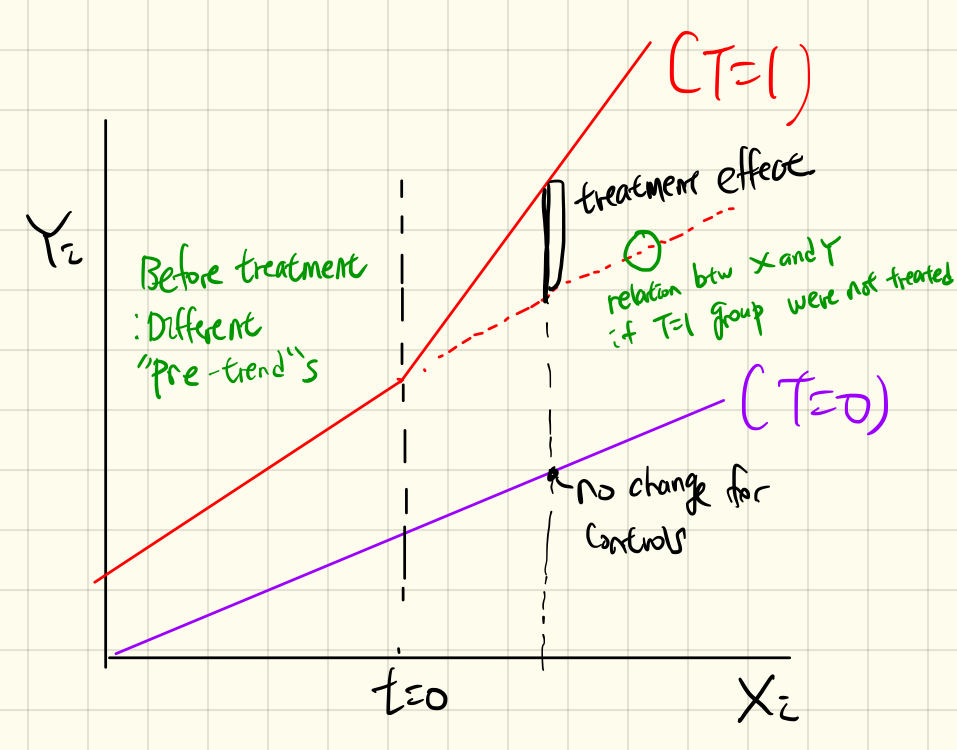
\includegraphics[width=\textwidth]{fig1_1.png}
\caption{No change in control group}
\end{subfigure}
\begin{subfigure}[b]{.45\textwidth}
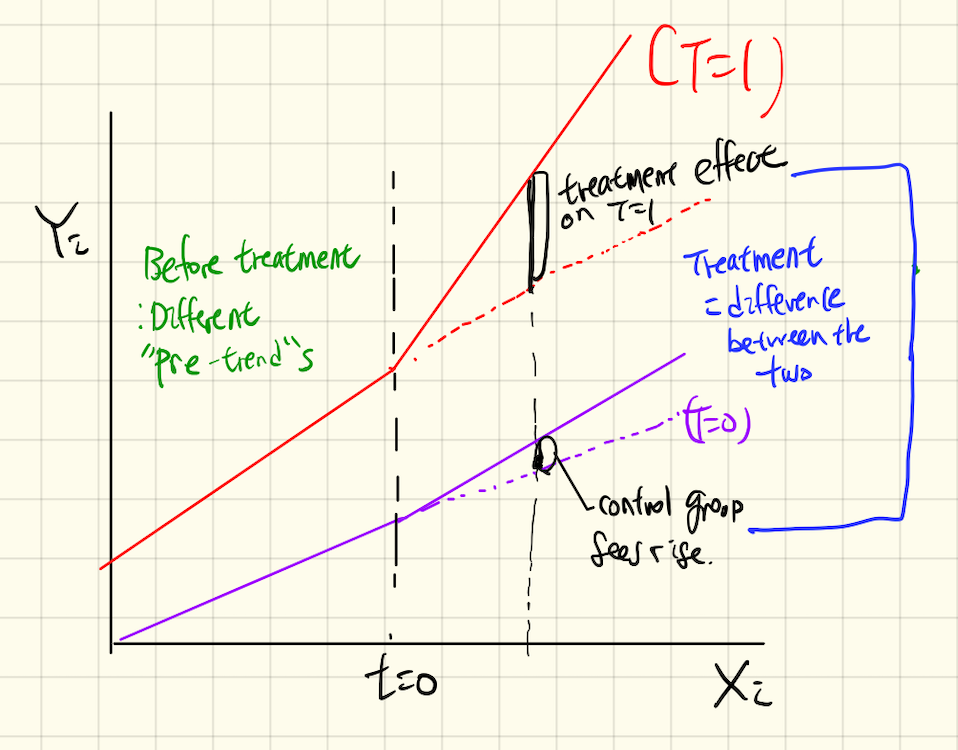
\includegraphics[width=\textwidth]{fig1_2.png}
\caption{Some change in control group}
\end{subfigure}
\end{figure}
\end{frame}

\begin{frame}
\frametitle{Regression discontinuity}
\begin{itemize}
\item This applies to case where the treatment status depends on a threshold
\item Loosely speaking, we have
\[
Y_i = \beta_0+\beta_1X_i+u_i
\]
where $X_i=1$ if $i$ passes threshold for eligibility (0 if otherwise)
\item Back out the treatment effect using the difference
\begin{itemize}
\item For those not in the program, $E[Y_i|X_i=0]=\beta_0$ 
\item For those in the program, $E[Y_i|X_i=1]=\beta_0+\beta_1$
\end{itemize}
\item Thus, $\beta_1$ is the treatment effect
\item Note: For RD to work, there should be no `jump' in observables around the threshold except treatment status
\item Loss of samples: RD is applied to a narrow bandwidth around the threshold
\item There may be cases where threshold is not strict (fuzzy RD)
\end{itemize}
\end{frame}

\begin{frame}
\frametitle{Regression discontinuity: In pictures}
\begin{figure}[H]
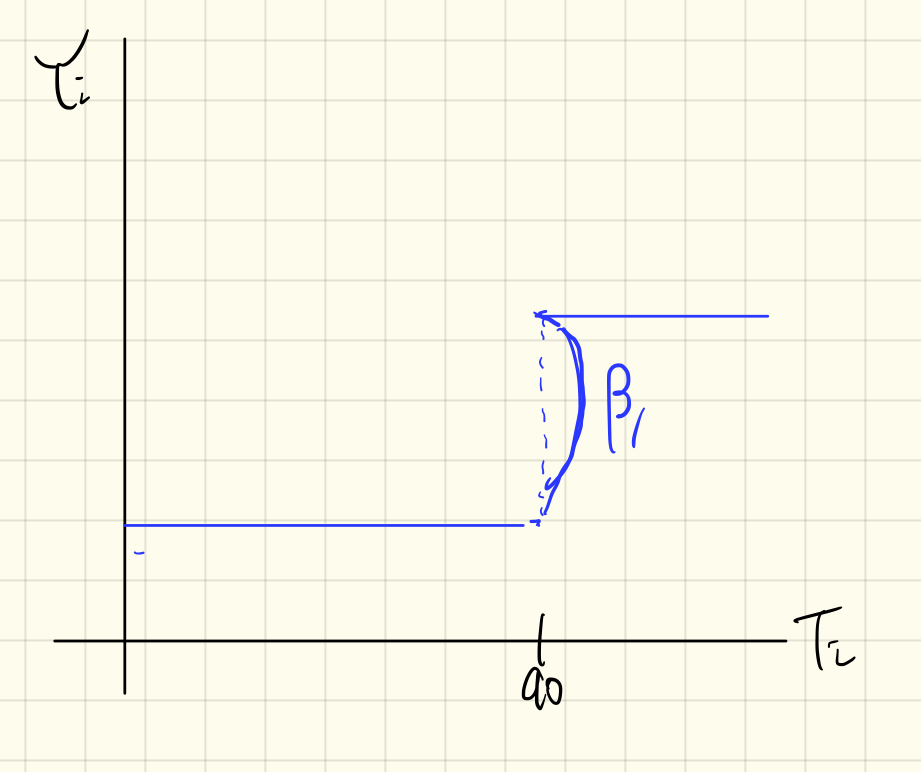
\includegraphics[width=0.6\textwidth, keepaspectratio]{fig2.png}
\end{figure}
\end{frame}
%%%%%%%%%%%
\end{document}
